\documentclass{article}

% NeurIPS submission-style template. Use the default option instead of
% preprint for double-blind submission; this report keeps authors visible.
\usepackage[preprint,nonatbib]{neurips_2026}

\usepackage[UTF8,scheme=plain]{ctex}
\usepackage{amsmath}
\usepackage{amssymb}
\usepackage{booktabs}
\usepackage{graphicx}
\usepackage{hyperref}
\usepackage{enumitem}
\usepackage{xcolor}

\hypersetup{
  colorlinks=true,
  linkcolor=blue!55!black,
  citecolor=blue!55!black,
  urlcolor=blue!55!black
}

\setlist[itemize]{leftmargin=*,topsep=2pt,itemsep=2pt}
\setlist[enumerate]{leftmargin=*,topsep=2pt,itemsep=2pt}
\graphicspath{{figures/}}
\emergencystretch=3em
\sloppy

\newcommand{\placeholder}[1]{\textcolor{gray}{\textbf{[待补充：#1]}}}
\newcommand{\method}[1]{\textsc{#1}}

\title{面向指令图像编辑的 Qwen-Image-Edit LoRA 适配与多专家教师构造}

\author{
  \begin{tabular}{c}
  王溢韬 \\
  \placeholder{单位/实验室名称} \\
  \texttt{\placeholder{邮箱}} \\
  \\
  \placeholder{共同作者姓名} \\
  \placeholder{单位/实验室名称} \\
  \texttt{\placeholder{邮箱}}
  \end{tabular}
}

\begin{document}

\maketitle

\begin{abstract}
本文围绕指令图像编辑任务，对 Qwen-Image-Edit-2511 基座模型在 MagicBrush 数据集上的任务适配进行系统梳理。报告首先建立统一的数据、训练与评测设定，然后比较未微调基座模型、基于真实目标图像的 GT LoRA、基于 mask-preserved target 的 MTP LoRA，以及基于多专家融合教师的 MoE Teacher LoRA。实验结果显示，GT LoRA 可将 MagicBrush-dev 上的 Target--Output SSIM 从 0.450 提升至 0.696；MTP LoRA 通过显式约束背景保持与编辑区域学习，将该指标进一步提升至 0.740；MoE Teacher LoRA 利用 Pix2Pix、Qwen-Image-Edit 与 EditAR 候选结果构造区域级 teacher，最终达到 0.763 的 Target--Output SSIM 与 0.852 的 BG-SSIM。总体而言，面向局部编辑任务的监督目标重构与区域级教师蒸馏，是提升图像编辑模型目标一致性与背景保持能力的有效途径。
\end{abstract}

\section{Introduction}

指令图像编辑要求模型在给定原始图像 $I$ 与文本指令 $p$ 的条件下生成编辑后图像 $O$。与纯文本到图像生成相比，该任务同时强调语义理解、局部编辑、空间定位与背景保持：模型既需要根据指令完成目标区域的语义变化，又应避免对无关区域产生不必要扰动。对于 MagicBrush 这类人工标注数据集，训练样本通常包含原图、文本指令、目标图像与编辑区域 mask，这为监督微调提供了直接依据，也带来了目标图像噪声、mask 极性不稳定、背景区域主导损失等实际问题。

本报告以 Qwen-Image-Edit-2511 作为基座模型，研究如何通过 LoRA 适配提升其在 MagicBrush 指令编辑任务上的表现。基座模型具有较强的通用语义理解能力，但在特定数据分布上仍存在编辑位置不够精确、背景保持不足等问题。为此，本文首先验证直接使用真实目标图像进行 LoRA 微调的有效性，再进一步提出两类改进：其一是 MTP（Masked Target Programming），通过构造保留背景的 clean target 缓解局部监督不清的问题；其二是 MoE-Fusion Teacher，通过多专家候选与区域级路由构造更高质量的训练期 teacher，并将其蒸馏到单一 Qwen2511 LoRA 模型中。

本文的主要内容包括：
\begin{itemize}
  \item 建立统一的指令图像编辑建模形式、数据协议与评测指标；
  \item 将 Qwen2511 Base、GT LoRA、MTP LoRA 与 MoE Teacher LoRA 置于同一实验框架下比较；
  \item 给出 MTP 的 mask 选择、目标重构与区域归一化损失设计；
  \item 给出 MoE-Fusion Teacher 的专家评分、区域路由、融合与蒸馏流程；
  \item 汇总 MagicBrush-dev 上的客观指标、MLLM 评测指标与定性观察。
\end{itemize}

\section{Related Works}

\paragraph{指令图像编辑。}
指令图像编辑模型通常将原图与自然语言指令共同作为条件，生成满足指令约束的编辑结果。InstructPix2Pix 证明了文本指令可以有效驱动扩散模型完成开放域图像编辑；MagicBrush 进一步提供人工标注的指令编辑数据，为监督训练与评测提供了更稳定的数据基础。本文工作沿用该任务设定，但重点关注在给定强基座模型后，如何通过更合理的监督目标与蒸馏策略提升局部编辑质量。

\paragraph{参数高效微调。}
LoRA 通过在冻结主干参数的前提下引入低秩可训练矩阵，实现参数高效的任务适配。对于大规模图像编辑模型，LoRA 能在显著降低训练成本的同时保留基座模型的通用生成能力。本文采用 LoRA 对 Qwen2511 的 DiT 模块进行适配，并比较不同监督目标对同一 LoRA 训练框架的影响。

\paragraph{区域感知训练与背景保持。}
局部图像编辑的关键难点之一是避免背景漂移。若直接对全图目标进行平均损失优化，大面积背景会主导梯度；若只强调编辑区域，又可能削弱全局一致性与边界自然度。因此，区域 mask、边界约束、背景保持损失以及 clean target 构造，是提升局部编辑稳定性的常见手段。本文提出的 MTP 将目标图与原图按照 soft mask 组合，把“编辑区域学习”和“背景区域保持”显式写入监督目标。

\paragraph{多专家融合与教师蒸馏。}
多专家方法通过组合不同模型或不同候选结果的优势，提高复杂任务上的鲁棒性。对于图像编辑，同一指令在不同区域可能更适合不同专家：部分专家更善于产生语义正确的编辑内容，部分专家更善于维持背景一致性。MoE-Fusion Teacher 在训练阶段利用 target 与 mask 对专家候选进行评分和区域路由，构造更高质量的 teacher，再通过 LoRA 蒸馏到单模型中，以保持推理阶段的部署简洁性。

\section{Problem Setup}

\subsection{数据与符号}

本文研究的指令图像编辑输入为原图 $I$ 与文本指令 $p$，输出为编辑图 $O$。监督数据来自 MagicBrush，每个样本记为：
\[
(I,p,G,M),
\]
其中 $G$ 为人工目标图像，$M\in\{0,1\}^{H\times W}$ 为编辑区域 mask。实验划分如下：
\begin{itemize}
  \item 训练集：MagicBrush train，共 8807 条样本；
  \item 测试集：MagicBrush dev，共 528 条样本；
  \item 图像尺寸：训练与推理使用 Qwen-Image-Edit-2511 图像编辑接口，最大像素数为 $512^2=262144$。
\end{itemize}

\subsection{统一建模形式}

所有可部署学生模型均遵循同一推理形式：
\[
O=f_{\theta}(I,p).
\]
训练数据在 DiffSynth/Qwen-Image-Edit 的 metadata 中统一写为：
\[
\texttt{edit\_image}=[I],\quad
\texttt{prompt}=p,\quad
\texttt{image}=Y,
\]
其中 $Y$ 为当前实验使用的监督目标。不同方法只改变 $Y$ 的定义：
\[
Y=
\begin{cases}
G, & \text{GT LoRA},\\
\bar G, & \text{MTP LoRA},\\
T_{\mathrm{moe}}, & \text{MoE Teacher LoRA}.
\end{cases}
\]
因此，各方法在推理阶段均保持相同接口：
\[
\texttt{input image}+\texttt{instruction}
\longrightarrow
\texttt{edited image}.
\]

\subsection{评测指标}

本文使用客观指标与 MLLM 辅助评测共同分析模型表现。客观指标包括 Target--Output SSIM、Target--Output PSNR、BG-SSIM、Input--Output SSIM、Input--Output PSNR 与 Edit Change。其中，Target--Output 指标衡量输出与目标图的一致性；BG-SSIM 衡量背景保持能力；Edit Change 衡量模型实际产生编辑变化的强度。MLLM 评测指标包括 Preference、Instruction、Background 与 Target，用于辅助观察语义遵循、背景保持和目标一致性。

\section{Methods}

\subsection{Qwen2511 Base}

首先评测不加载任何 LoRA 的 Qwen-Image-Edit-2511：
\[
O=f_{\theta_0}(I,p).
\]
该基座模型具备较强的语言理解和通用编辑先验，对多数指令能够产生基本响应；但由于未针对 MagicBrush 监督分布进行适配，输出仍容易出现编辑位置偏移、局部替换不完整和背景扰动。该模型在 MagicBrush-dev 上的 Target--Output SSIM 为 0.450，Target--Output PSNR 为 14.29。

\subsection{GT LoRA}

GT LoRA 直接使用人工目标图 $G$ 作为监督目标，以验证 Qwen2511 在 MagicBrush 分布上的可适配性。LoRA 冻结 Qwen2511 原始 DiT 权重 $W_0$，并在目标线性层上加入低秩更新：
\[
W'=W_0+\Delta W,\qquad
\Delta W=\frac{\alpha}{r}BA,
\]
其中 $A\in\mathbb{R}^{r\times d}$，$B\in\mathbb{R}^{k\times r}$，$r$ 为 LoRA rank，$\alpha$ 为缩放系数。训练时只更新 LoRA 参数：
\[
\theta^\star_{\mathrm{LoRA}}
=
\arg\min_{\theta_{\mathrm{LoRA}}}
\mathbb{E}_{(I,p,G,M)}
\left[
\mathcal{L}(f_{\theta_0,\theta_{\mathrm{LoRA}}}(I,p),G,M)
\right].
\]
本文实验中，LoRA 注入 Qwen2511 DiT 的 attention 与 modulation/MLP 层；GT LoRA 使用 rank 32，学习率 $1\times10^{-4}$，训练 1 个 epoch，采用 4 张 A100 并行。若精确硬件、batch size 或 scheduler 配置需作为投稿附录公开，可在此补充：\placeholder{完整训练超参数}。

\subsection{训练流程与 Mask-aware 流匹配损失}

Qwen-Image-Edit-2511 的训练管线可抽象为文本编码器、图像 VAE、扩散 DiT 与调度器四部分。对样本 $(I,p,Y,M,w_s)$，首先用 VAE 编码目标图与条件图：
\[
z_Y=\operatorname{Enc}_{\mathrm{vae}}(Y),\qquad
z_I=\operatorname{Enc}_{\mathrm{vae}}(I),
\]
并由文本编码器得到指令表示：
\[
h_p=\operatorname{Enc}_{\mathrm{text}}(p).
\]
随后对目标隐变量 $z_Y$ 采样时间步 $t$ 与噪声 $\epsilon$，得到：
\[
z_t=a(t)z_Y+b(t)\epsilon.
\]
DiT 接收加噪隐变量、文本条件与图像条件，预测速度场：
\[
\hat u_t
=
D_{\theta_0+\Delta\theta}(z_t,t,h_p,z_I).
\]
优化目标为：
\[
\Delta\theta^\star
=
\arg\min_{\Delta\theta}
\mathbb{E}
\left[
\mathcal{L}_{\mathrm{region}}(\hat u_t,u_t,M,w_s)
\right],
\]
其中 $\Delta\theta$ 表示所有 LoRA adapter 参数。

为避免全图平均损失被大面积背景主导，本文将编辑 mask resize 到隐变量尺度，记为 $\hat M$，背景为 $\hat B=1-\hat M$，逐元素误差为：
\[
E=\left\|v_\theta(z_t,t,I,p)-v^\star\right\|_2^2.
\]
区域归一化损失定义为：
\[
\mathcal{L}_{\mathrm{edit}}=\frac{\sum \hat M E}{\sum \hat M+\varepsilon},\qquad
\mathcal{L}_{\mathrm{bg}}=\frac{\sum \hat B E}{\sum \hat B+\varepsilon}.
\]
GT LoRA 的最终损失为：
\[
\mathcal{L}_{\mathrm{sft}}
=
w_s\cdot
\frac{\lambda_e\mathcal{L}_{\mathrm{edit}}+\lambda_b\mathcal{L}_{\mathrm{bg}}}
{\lambda_e+\lambda_b},
\]
默认使用 $\lambda_e=1.5,\lambda_b=0.5$。该设计使编辑区域的梯度不会被背景像素数量淹没。

\begin{figure}[t]
\centering
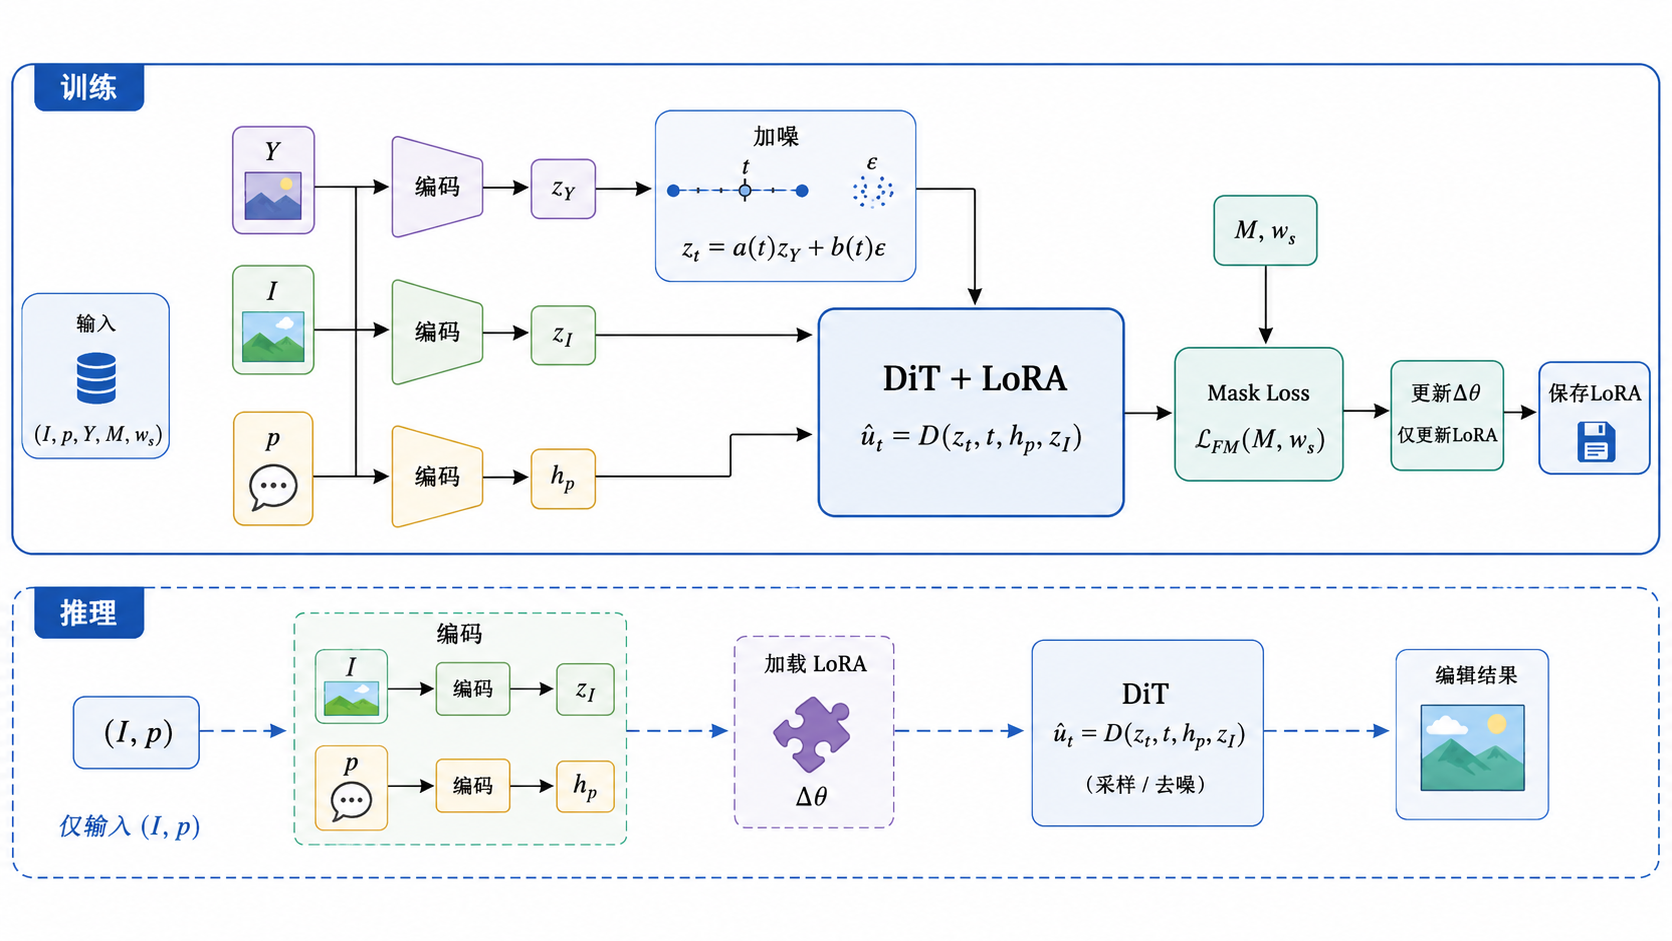
\includegraphics[width=\linewidth]{gt_lora.png}
\caption{GT LoRA 的训练框架。}
\label{fig:gt-lora}
\end{figure}

\subsection{MTP LoRA}

MTP（Masked Target Programming）的核心思想是不直接拟合整张目标图 $G$，而是构造更适合局部编辑学习的 clean target：
\[
\bar G=\tilde M\odot G+(1-\tilde M)\odot I,
\]
其中 $\tilde M\in[0,1]^{H\times W}$ 为 soft edit mask。该目标在编辑区域保留人工目标图，在背景区域回退到原图，从而显式约束模型不要修改无关区域。

\paragraph{Mask 生成与选择。}
MTP 同时考虑 source-target diff mask、数据集 mask 与反相数据集 mask：
\[
\mathcal{M}=
\{M_{\mathrm{diff}}, M_{\mathrm{dataset}}, 1-M_{\mathrm{dataset}}\}.
\]
source-target 差异图定义为：
\[
D(i,j)=\frac{1}{3}\sum_c |I(i,j,c)-G(i,j,c)|.
\]
对差异图使用 Otsu 阈值或固定阈值生成初始 diff mask，并经过移除小连通域、填洞、闭运算与膨胀等形态学清理。对候选 mask $M$，定义面积、区域内外差异和覆盖率：
\[
a(M)=\frac{1}{HW}\sum_{i,j}M_{ij},
\]
\[
d_{\mathrm{in}}(M)=\frac{\sum M\odot D}{\sum M+\varepsilon},\qquad
d_{\mathrm{out}}(M)=\frac{\sum (1-M)\odot D}{\sum (1-M)+\varepsilon},
\]
\[
c(M)=\frac{\sum M\odot D}{\sum D+\varepsilon}.
\]
最终评分为：
\[
S_M(M)=
d_{\mathrm{in}}(M)-d_{\mathrm{out}}(M)
+\beta c(M)
-\gamma\max(0,a(M)-a_{\mathrm{broad}})
-\eta\max(0,a_{\mathrm{tiny}}-a(M)).
\]
选择最高分候选作为 $M^\star$。若指令属于全局编辑，或 mask 面积超过阈值，则允许使用全图编辑，令 $\tilde M=\mathbf{1}$。

\paragraph{Soft mask 与 clean target。}
MTP 先对 $M^\star$ 膨胀，再进行高斯 feather：
\[
M_d=\operatorname{Dilate}(M^\star,r_d),
\qquad
\tilde M=\operatorname{clip}\left(\mathcal{G}_{\sigma}*M_d,0,1\right).
\]
边界 mask 定义为：
\[
M_{\mathrm{bd}}
=
\operatorname{Dilate}(M^\star,r_{\mathrm{bd}})
-
\operatorname{Erode}(M^\star,r_{\mathrm{bd}}).
\]
随后使用 $\bar G$ 替代 $G$ 作为训练目标。为增强保持能力，MTP 每隔固定 stride 加入 no-op 样本：
\[
I+\text{``Do not change the image''}\rightarrow I.
\]
这类样本的 mask 为全 0，样本权重较低，只作为保持能力正则。

\paragraph{MTP 损失。}
MTP 使用 clean target $\bar G$ 的隐变量作为流匹配监督，并引入编辑区、背景区和边界区三项区域归一化损失：
\[
\mathcal{L}_{\mathrm{mtp}}
=
\frac{
\lambda_e\mathcal{L}_{\mathrm{edit}}
+\lambda_b\mathcal{L}_{\mathrm{bg}}
+\lambda_{\mathrm{bd}}\mathcal{L}_{\mathrm{bd}}}
{\lambda_e+\lambda_b+\lambda_{\mathrm{bd}}},
\]
其中：
\[
\mathcal{L}_{\mathrm{bd}}
=
\frac{\sum \hat M_{\mathrm{bd}} E}{\sum \hat M_{\mathrm{bd}}+\varepsilon}.
\]
最终采用的 PhaseA 设置为 $\lambda_e=4.0,\lambda_b=0.3,\lambda_{\mathrm{bd}}=0.15$，LoRA rank 为 16，学习率为 $5\times10^{-5}$，训练 1 个 epoch。

\begin{figure}[t]
\centering
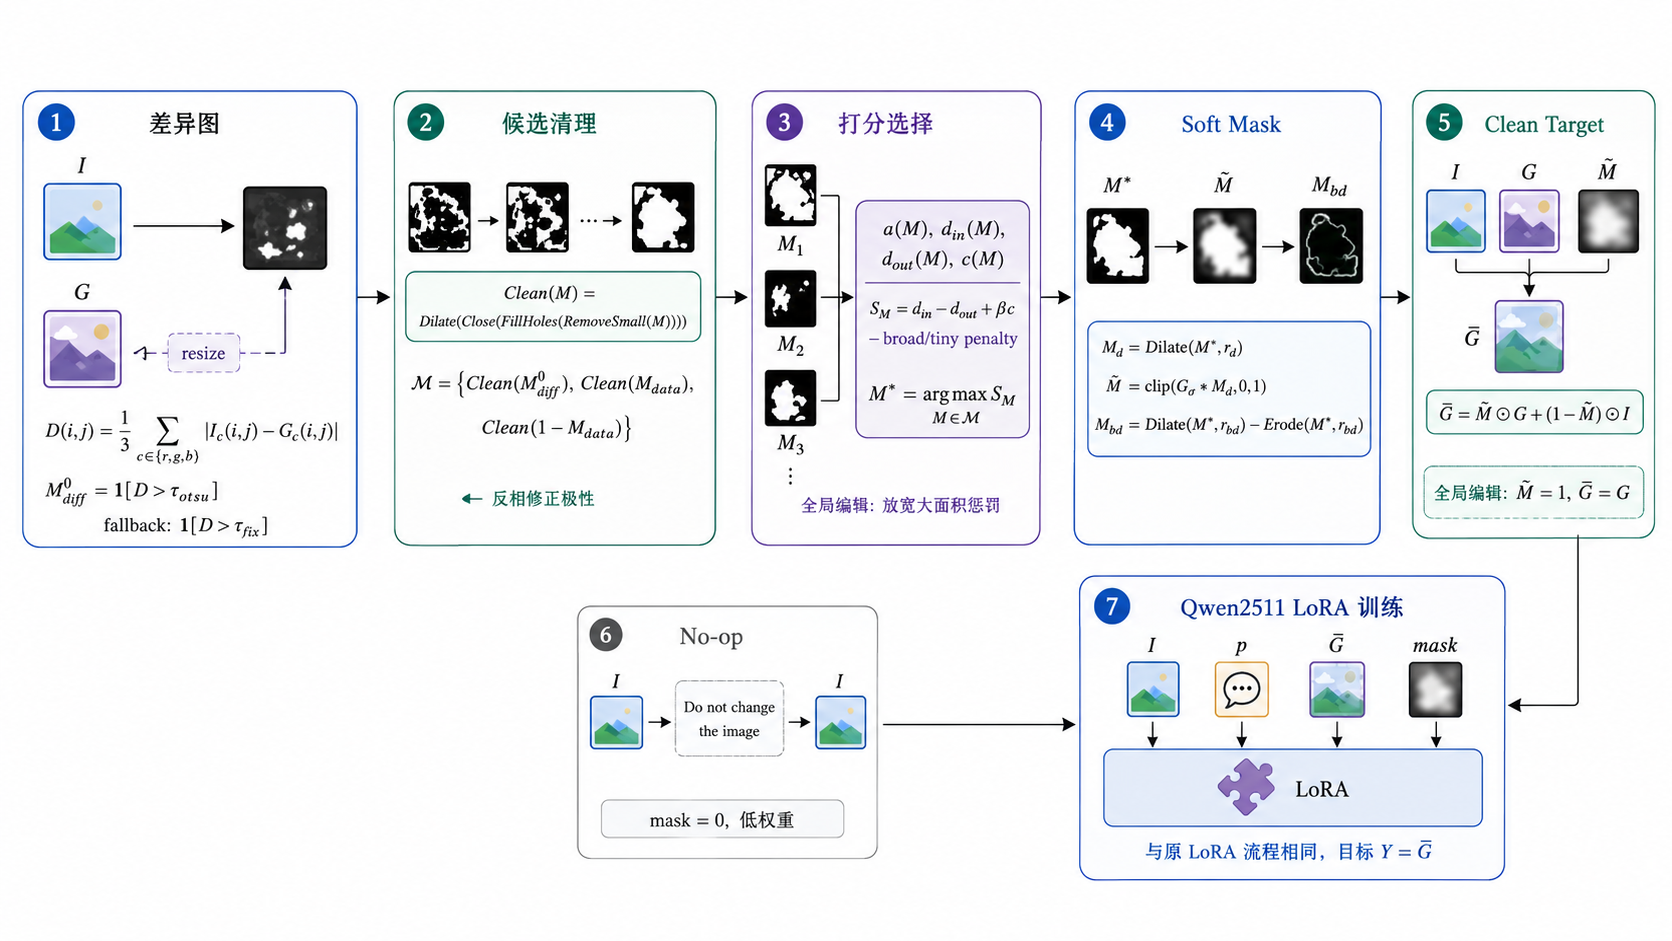
\includegraphics[width=\linewidth]{mtp_lora.png}
\caption{MTP LoRA 的训练目标构造与微调流程。}
\label{fig:mtp-lora}
\end{figure}

\subsection{MoE-Fusion Teacher}

MoE-Fusion Teacher 的目标是在训练阶段利用多个专家的候选结果构造更高质量的 teacher。候选集合为：
\[
\mathcal{C}=\{C_{\mathrm{pix2pix}},C_{\mathrm{qwen}},C_{\mathrm{editar}}\}.
\]
实际实现中，Qwen 候选额外生成 conservative 与 aggressive 两个虚拟变体：
\[
C_{\mathrm{qwen\mbox{-}cons}}
=
\operatorname{clip}\left(I+s_c(C_{\mathrm{qwen}}-I),0,1\right),
\qquad s_c=0.65,
\]
\[
C_{\mathrm{qwen\mbox{-}aggr}}
=
\operatorname{clip}\left(I+s_a(C_{\mathrm{qwen}}-I),0,1\right),
\qquad s_a=1.25.
\]
因此实际路由专家族为：
\[
\mathcal{E}
=
\{\text{pix2pix},\text{qwen},\text{qwen-cons},\text{qwen-aggr},\text{editar}\}.
\]

\paragraph{专家评分。}
对每个候选 $C$，分别计算编辑区目标相似、背景保持、方向一致性与边界自然度：
\[
E_{\mathrm{edit}}(C)=\operatorname{MSE}(C,G;M)
+\alpha_s\left(1-\operatorname{SSIM}(C,G;M)\right),
\]
\[
E_{\mathrm{bg}}(C)=\operatorname{MSE}(C,I;1-M)
+\alpha_b\left(1-\operatorname{SSIM}(C,I;1-M)\right),
\]
\[
D_{\mathrm{dir}}(C)=1-\cos\left((C-I)\odot M,(G-I)\odot M\right),
\]
\[
B(C)=
\rho\|C-I\|_{1,M_{\mathrm{bd}}}
+(1-\rho)\|\nabla C-\nabla I\|_{1,M_{\mathrm{bd}}}.
\]
综合得分越低越好：
\[
S(C)=
\lambda_e E_{\mathrm{edit}}(C)
+\lambda_b E_{\mathrm{bg}}(C)
+\lambda_d D_{\mathrm{dir}}(C)
+\lambda_{\mathrm{bd}}B(C)
+\lambda_f\operatorname{MSE}(C,G).
\]

\paragraph{区域级路由与融合。}
MoE 将编辑 mask 分解为连通区域：
\[
M=\bigcup_{k=1}^{K}M_k,
\]
每个区域独立选择专家：
\[
e_k^\star
=
\arg\min_{e\in\mathcal{E}} S_k(C_e).
\]
当最优专家明显优于第二名时执行硬路由；若多个专家质量接近，则在 top-$K$ 专家之间做软路由：
\[
\pi_{k,e}
=
\frac{\exp(-S_k(C_e)/\tau)}
{\sum_{e'\in\operatorname{TopK}(k)}\exp(-S_k(C_{e'})/\tau)},
\qquad
C_k^{\mathrm{route}}=\sum_{e\in\operatorname{TopK}(k)}\pi_{k,e}C_e.
\]
局部编辑样本默认使用 source 作为背景专家，即 $C_{\mathrm{bg}}=I$。初始融合图为：
\[
T_0
=
(1-\tilde M)\odot C_{\mathrm{bg}}
+\sum_{k=1}^{K}\tilde M_k\odot C_{e_k^\star}.
\]
随后执行颜色协调化与拉普拉斯融合，得到 teacher：
\[
T_{\mathrm{moe}}=\operatorname{Blend}_{\mathrm{lap}}(\operatorname{Harmonize}(T_0,I,M)).
\]
若融合结果的综合评分显著差于最佳单专家，则回退到最佳单专家，以避免 teacher 退化。

\paragraph{Teacher 蒸馏。}
MoE teacher 只用于训练目标，学生仍为 Qwen2511 source-only LoRA。样本权重由 teacher confidence 调节：
\[
w_s=\operatorname{clip}(w_{\min}+\operatorname{conf}(T_{\mathrm{moe}})(w_{\max}-w_{\min}),w_{\min},w_{\max}).
\]
训练损失为：
\[
\mathcal{L}_{\mathrm{moe}}=w_s
\frac{\lambda_e\mathcal{L}_{\mathrm{edit}}^{\mathrm{moe}}
+\lambda_b\mathcal{L}_{\mathrm{bg}}^{\mathrm{moe}}}
{\lambda_e+\lambda_b}.
\]
其定义与 GT LoRA 相同，但监督目标由 $G$ 替换为 $T_{\mathrm{moe}}$。

\begin{figure}[t]
\centering
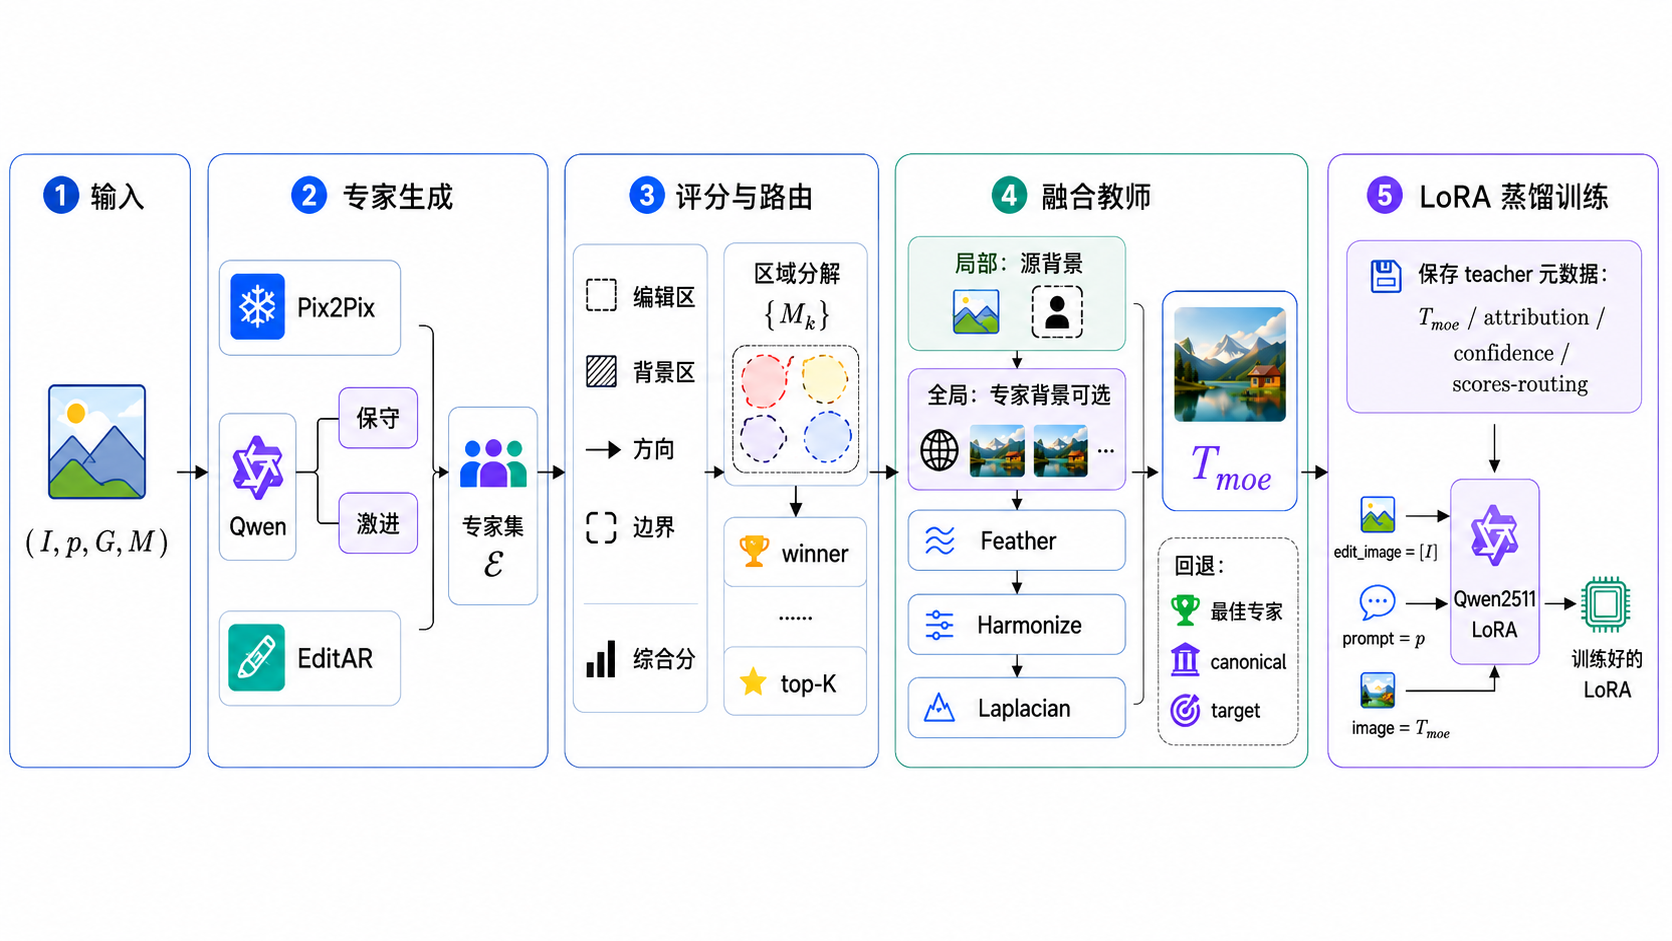
\includegraphics[width=\linewidth]{moe_lora.png}
\caption{MoE Teacher LoRA 的多专家 teacher 构造与学生蒸馏流程。}
\label{fig:moe-lora}
\end{figure}

\section{Results}

\subsection{客观指标}

\begin{table}[t]
\centering
\small
\caption{MagicBrush-dev 客观指标。TO 表示 Target--Output，IO 表示 Input--Output。MoE Teacher 为训练期 teacher，其他 LoRA 方法为可部署学生模型。}
\label{tab:objective-release}
\resizebox{\linewidth}{!}{%
\begin{tabular}{lrrrrrr}
\toprule
Method & TO SSIM$\uparrow$ & TO PSNR$\uparrow$ & BG-SSIM$\uparrow$ & IO SSIM$\uparrow$ & IO PSNR$\uparrow$ & Edit Change \\
\midrule
Qwen2511 Base & 0.450 & 14.29 & 0.696 & 0.450 & 14.37 & 0.135 \\
GT LoRA & 0.696 & 18.24 & 0.821 & 0.702 & 18.42 & 0.043 \\
MTP LoRA & 0.740 & 18.46 & 0.828 & 0.761 & 19.38 & 0.172 \\
MoE Teacher & 0.881 & 22.84 & 0.993 & 0.951 & 29.25 & 0.115 \\
MoE Teacher LoRA & \textbf{0.763} & \textbf{19.01} & \textbf{0.852} & \textbf{0.792} & \textbf{20.02} & 0.167 \\
\bottomrule
\end{tabular}%
}
\end{table}


从表~\ref{tab:objective-release} 可以看出，直接使用 GT LoRA 已能显著提升目标一致性，说明 Qwen2511 对 MagicBrush 分布具有良好的参数高效适配空间。MTP LoRA 在 Target--Output SSIM、BG-SSIM 与 Edit Change 上均优于 GT LoRA，表明 clean target 能同时提升编辑发生强度与背景保持质量。MoE Teacher LoRA 在可部署学生模型中取得最高 Target--Output SSIM、Target--Output PSNR 与 BG-SSIM，说明区域级 teacher 对学生微调提供了更高质量的监督信号。

\subsection{MLLM 评测}

\begin{table}[t]
\centering
\small
\caption{MagicBrush-dev Qwen3-VL/MLLM 评测指标。MoE Teacher 未运行 MLLM，因此不列入该表。}
\label{tab:mllm-release}
\resizebox{\linewidth}{!}{%
\begin{tabular}{lrrrr}
\toprule
Method & Preference$\uparrow$ & Instruction$\uparrow$ & Background$\uparrow$ & Target$\uparrow$ \\
\midrule
Qwen2511 Base & 7.07 & 9.23 & 9.29 & 8.85 \\
GT LoRA & 6.88 & 8.81 & 9.27 & 8.49 \\
MTP LoRA & 6.75 & 8.72 & 9.18 & 8.25 \\
\bottomrule
\end{tabular}%
}
\end{table}


MLLM 评测结果显示，Qwen2511 Base 在通用语义维度上仍具备较强表现；LoRA 微调后的模型在客观像素指标上提升明显，但部分 MLLM 偏好指标并未同步提升。这提示后续需要在像素级目标一致性之外，引入更强的语义质量控制、区域偏好学习或人工偏好对齐，以减少“指标提升但感知偏好下降”的情况。

\subsection{定性分析}

\begin{figure}[t]
\centering
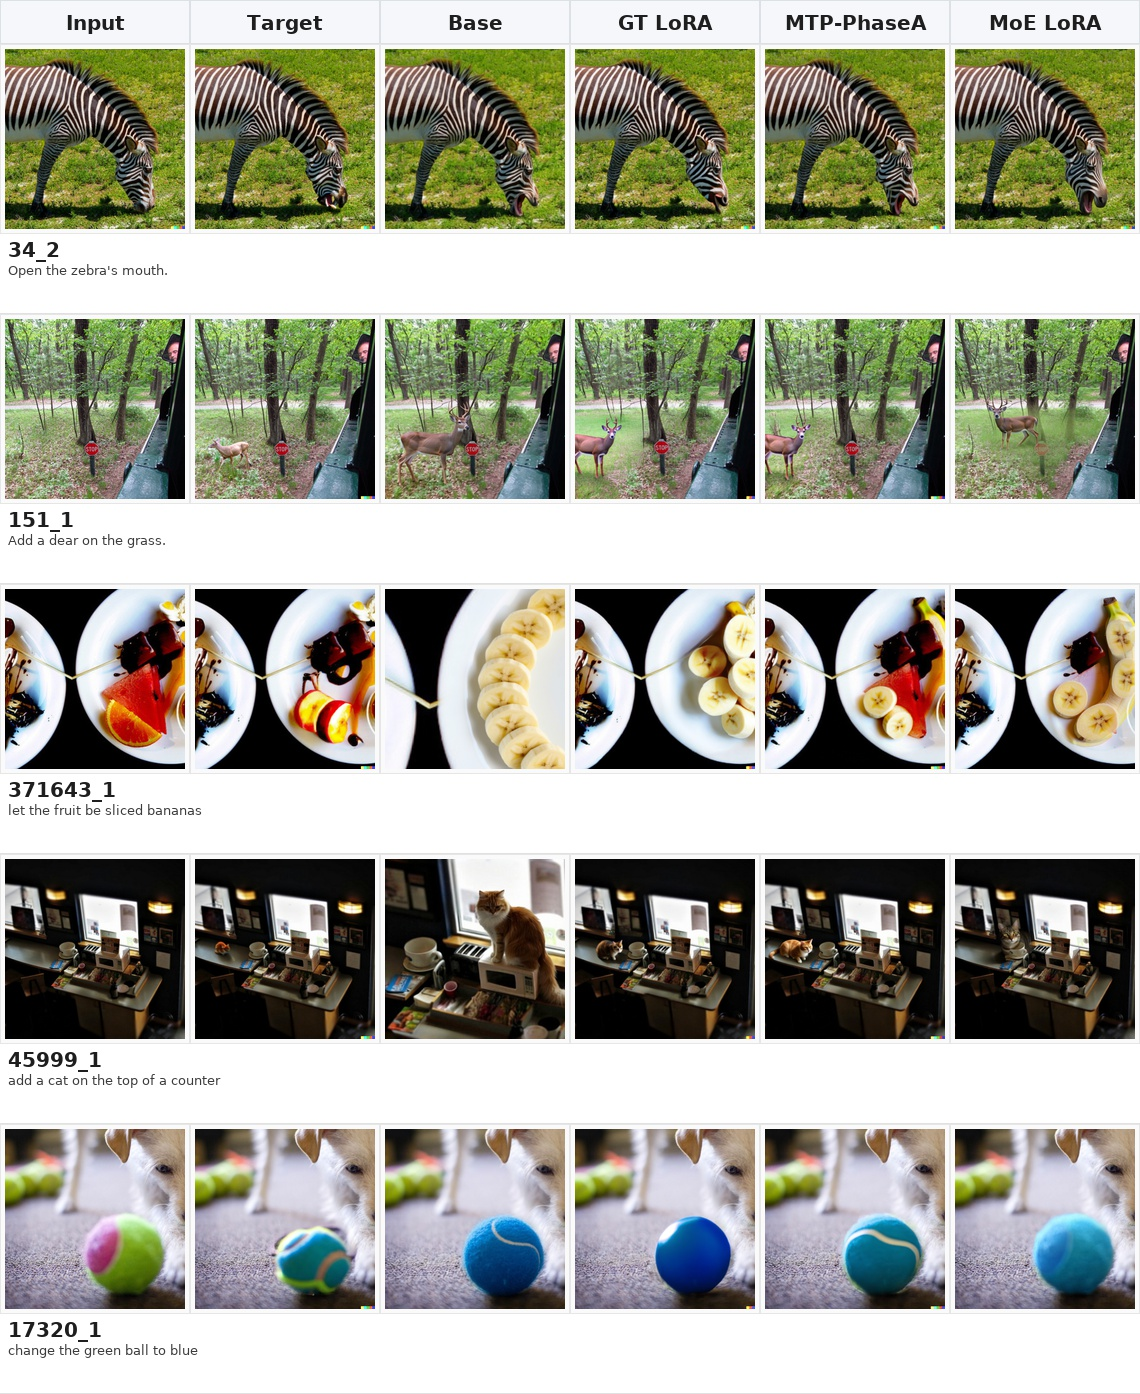
\includegraphics[width=\linewidth]{qwen2511_lora_failure_and_improvement_cases.jpg}
\caption{MagicBrush-dev 样例的定性对比。GT LoRA 相比 base 更能响应文本语义，但局部位置和背景保持仍存在不足；MTP 与 MoE Teacher LoRA 在局部约束与背景保持方面有进一步改进。}
\label{fig:case-comparison}
\end{figure}

\begin{figure}[t]
\centering
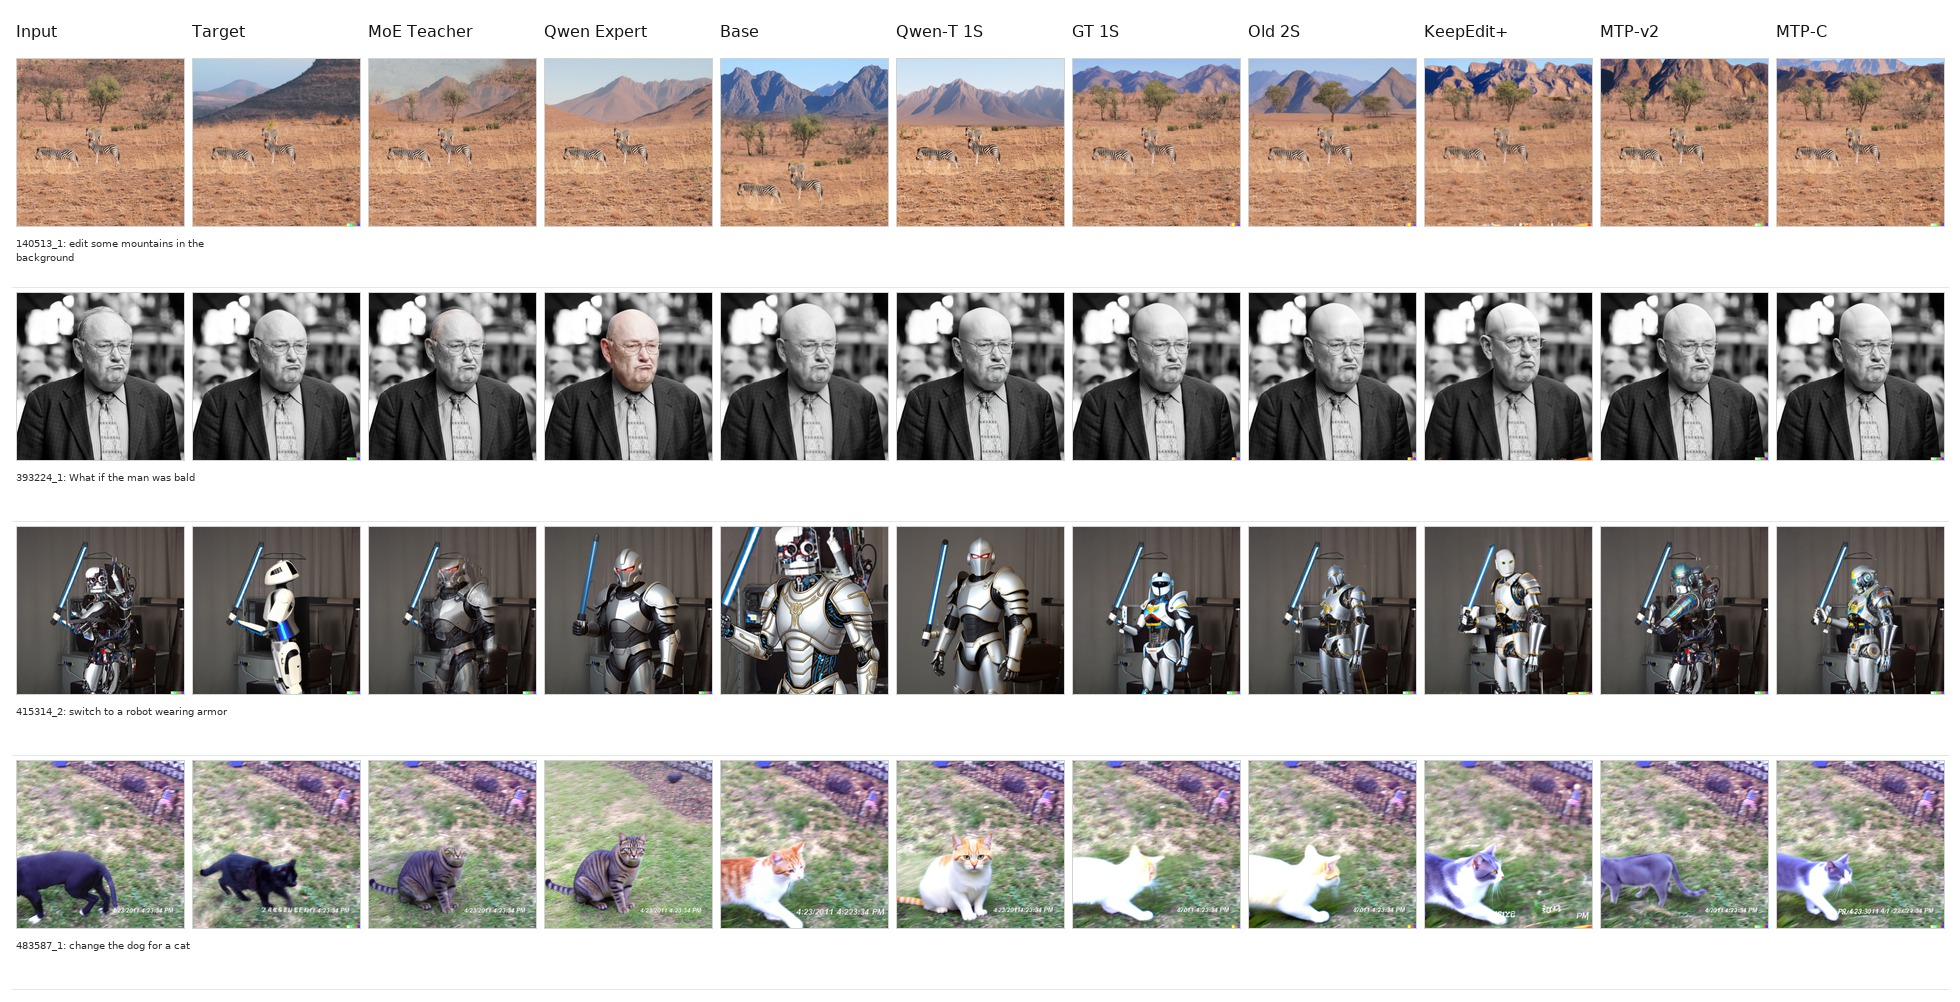
\includegraphics[width=\linewidth]{release_qualitative_comparison_grid.jpg}
\caption{发布版定性对比网格。该图用于展示不同模型在编辑完成度、局部一致性和背景保持方面的差异。}
\label{fig:release-grid}
\end{figure}

定性结果表明，GT LoRA 能改善基座模型对文本指令的响应，但在目标区域定位和背景稳定性上仍可能失败。例如，当目标对象替换需要精确空间定位时，GT LoRA 可能生成语义正确但位置不稳定的结果；当背景纹理复杂时，模型可能改变本应保持不变的区域。MTP 通过 clean target 明确将背景区域回写为原图，能有效缓解背景漂移；MoE Teacher LoRA 则进一步利用多专家候选，在部分样例中获得更自然的局部编辑结果。

\section{Discussion and Limitations}

当前结果可概括为四点。第一，Qwen2511 Base 的通用编辑能力较强，但未经任务适配时目标相似度偏低，且容易影响无关区域。第二，GT LoRA 证明了 MagicBrush 监督数据对大模型微调具有明显收益。第三，MTP 通过目标编程显式表达局部编辑与背景保持需求，在目标一致性与背景保持之间取得更好平衡。第四，MoE-Fusion Teacher 能提升训练信号质量，但仍受到专家候选质量差异的限制；当弱专家存在重影或语义错误时，融合结果可能将局部缺陷传递给学生模型。

后续工作可从以下方向继续推进：
\begin{itemize}
  \item 引入更强的语义 mask，例如 GroundingDINO、SAM 或 VLM planner，以提升编辑区域定位质量；
  \item 在 MoE 融合后加入扩散式局部 refinement，缓解边界不自然和弱专家伪影；
  \item 将 MoE 产生的区域级 winner/loser 信息转化为 preference loss，使学生学习区域选择偏好；
  \item 替换或扩展专家池，引入质量更稳定的扩散式编辑模型，提高 teacher 上限。
\end{itemize}

\section{Team Contributions}

\begin{table}[h]
\centering
\small
\caption{作者与团队分工。待确认成员以占位形式保留。}
\label{tab:team-contributions}
\begin{tabular}{p{0.18\linewidth}p{0.72\linewidth}}
\toprule
成员 & 主要职责 \\
\midrule
王溢韬 & 项目负责人；负责问题定义、Qwen2511 基座评测、LoRA 微调方案设计、MTP 目标构造、MoE-Fusion Teacher 设计、实验分析与技术报告撰写。 \\
\placeholder{成员姓名} & \placeholder{数据清洗、实验运行、可视化或消融实验职责} \\
\placeholder{成员姓名} & \placeholder{指标评测、人工评估、论文校对或复现实验职责} \\
\bottomrule
\end{tabular}
\end{table}

\section{Conclusion}

本文对 Qwen-Image-Edit-2511 在 MagicBrush 指令图像编辑任务上的 LoRA 适配进行了系统整理。实验表明，直接使用人工目标图训练 GT LoRA 已能显著提升任务表现；进一步通过 MTP 构造背景保持的 clean target，可提升局部编辑稳定性；通过 MoE-Fusion Teacher 构造区域级训练目标并蒸馏到单 LoRA 模型中，则能在目标一致性与背景保持上取得当前最佳结果。整体来看，面向局部图像编辑的高质量监督目标构造，是释放强基座模型任务适配能力的关键。

\begin{thebibliography}{9}

\bibitem{brooks2023instructpix2pix}
Tim Brooks, Aleksander Holynski, and Alexei A. Efros.
\newblock InstructPix2Pix: Learning to Follow Image Editing Instructions.
\newblock In CVPR, 2023.

\bibitem{zhang2023magicbrush}
Kai Zhang et al.
\newblock MagicBrush: A Manually Annotated Dataset for Instruction-Guided Image Editing.
\newblock NeurIPS Datasets and Benchmarks Track, 2023.

\bibitem{hu2021lora}
Edward J. Hu et al.
\newblock LoRA: Low-Rank Adaptation of Large Language Models.
\newblock arXiv:2106.09685, 2021.

\bibitem{isola2017pix2pix}
Phillip Isola, Jun-Yan Zhu, Tinghui Zhou, and Alexei A. Efros.
\newblock Image-to-Image Translation with Conditional Adversarial Networks.
\newblock In CVPR, 2017.

\bibitem{ho2020ddpm}
Jonathan Ho, Ajay Jain, and Pieter Abbeel.
\newblock Denoising Diffusion Probabilistic Models.
\newblock In NeurIPS, 2020.

\bibitem{lipman2023flow}
Yaron Lipman et al.
\newblock Flow Matching for Generative Modeling.
\newblock In ICLR, 2023.

\bibitem{kirillov2023sam}
Alexander Kirillov et al.
\newblock Segment Anything.
\newblock In ICCV, 2023.

\bibitem{shazeer2017moe}
Noam Shazeer et al.
\newblock Outrageously Large Neural Networks: The Sparsely-Gated Mixture-of-Experts Layer.
\newblock In ICLR, 2017.

\end{thebibliography}

\end{document}
